\documentclass{article}
\usepackage[backend=biber,natbib=true,style=authoryear]{biblatex}
\addbibresource{~/1_PROJECT/Bibliography.bib}
\usepackage[utf8]{inputenc}
\usepackage{graphicx}
\usepackage[colorlinks=true,linkcolor=blue,urlcolor=red,citecolor=magenta]{hyperref}
\usepackage{amsmath,amssymb,amsthm}
\allowdisplaybreaks
\numberwithin{equation}{section}
\newtheorem{assumption}{Assumption}[section]
\newtheorem{lemma}{Lemma}[section]
\newtheorem{corollary}{Corollary}[section]
\newtheorem{definition}{Definition}[section]
\newtheorem{proposition}{Proposition}[section]
\newtheorem{theorem}{Theorem}[section]
\newtheorem{notation}{Notation}[section]
\newtheorem{remark}{Remark}[section]
\newtheorem{example}{Example}[section]
\newtheorem{ques}{Question}[section]
\newtheorem{problem}{Problem}[section]
\newtheorem{conjecture}{Conjecture}[section]
\usepackage[left=0.5in,right=0.5in,top=1.5cm,bottom=1.5cm]{geometry}

\title{Optimal shape design of air ducts}
\author{Hong Nguyen}
\date{\today}

\begin{document}
\maketitle

Shape optimization has proved its indispensability from both theoretical and application points of view in many real world applications [1, 2, 4], such as drag reduction of aircrafts, designs of pipelines, bridges, engine components, implants for blood vessels, etc. For many optimal design problems in engineering or biomedical sciences, an optimal shape of a component or a device is determined to minimize some suitable objectives subject to fluid flows.

In the automotive industry particularly, the optimal shape design of several components of combustion engines, such as air ducts, piston, crankshaft, valves, etc., is crucial for their performance optimization. Additionally, the possible design is restricted by some geometric constraints.

To describe this problem mathematically, we use the stationary Navier-Stokes equation
\begin{equation}
\tag{NSEs}
\left\{\begin{split}
({\bf u}\cdot\nabla){\bf u} - \nu\Delta{\bf u} + \nabla p &= {\bf f} &&\mbox{ in } \Omega,\\
\nabla\cdot{\bf u} &= 0 &&\mbox{ in } \Omega,\\
{\bf u} &= {\bf f}_{\rm in} &&\mbox{ on inlet } \Gamma_{\rm i},\\
{\bf u} &= {\bf 0} &&\mbox{ on wall } \Gamma_{\rm w},\\
-\nu\partial_{\bf n}{\bf u} + p{\bf n} &= {\bf 0} &&\mbox{ on outlet } \Gamma_{\rm o},
\end{split}\right.
\end{equation}
to model the air flow inside a tube illustrated by the following figure:
\begin{figure}[h]
    \centering
    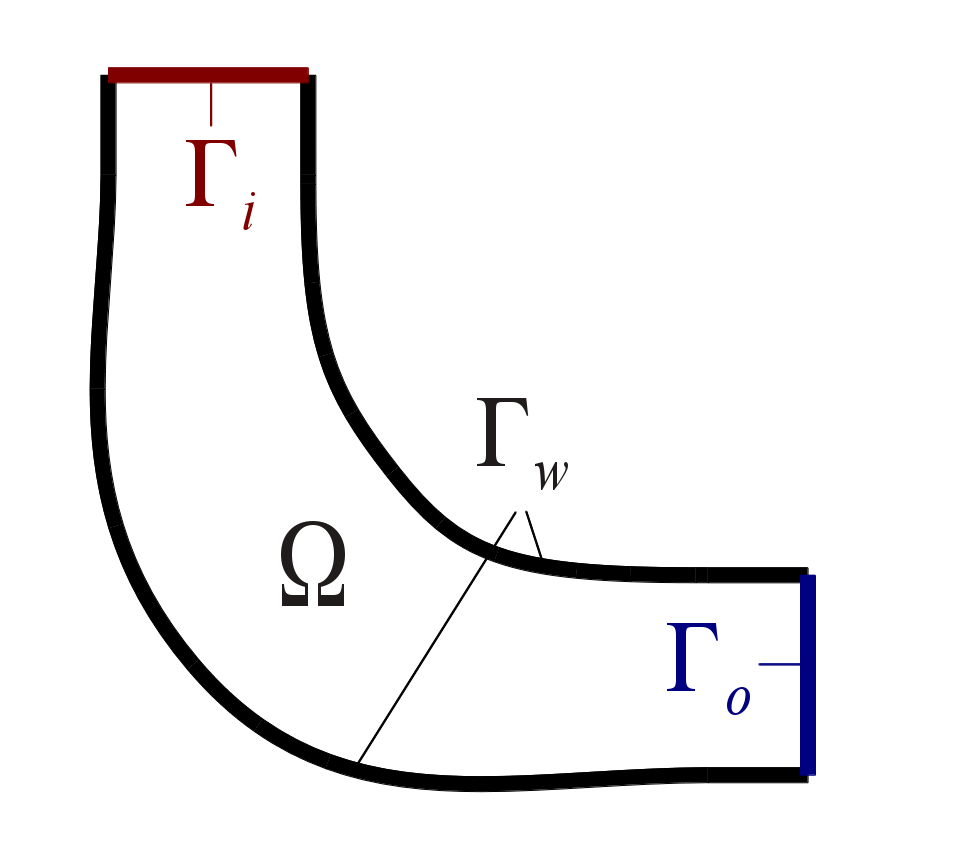
\includegraphics[scale=0.5]{geometrie_skizze_simple}
\end{figure}

Here ${\bf f}$ and ${\bf f}_{\rm in}$ are the given source density and inflow profile, $u$ and $p$ are the velocity and the kinematic pressure, ${\bf n}$ is the unit outward normal vector.

The uniformity of the flow leaving the outlet is an important design criterion of automotive air ducts to enhance the efficiency of distributing the air flow [2]. To achieve this criterion, we minimize a cost functional capturing the distance between the velocity (or only its normal component) and a given desired velocity in the outlet. Another criterion engineers also want to minimize is the power dissipated by air ducts (and any fluid dynamic devices in general) [2]. This dissipated power can be computed as the net inward flux of energy through the boundary of the considered tube.

Taking into account both objectives, we consider a mixed cost functional as a convex combination of the  cost functionals above. A typical PDE-constrained shape optimization problem [1, 4] can be established by finding an admissible shape to minimize the mixed cost functional under the given Navier-Stokes equation. After setting up our optimization problem, the optimal shape of the tube can be analyzed with some suitable methods based on shape derivatives.

Furthermore, large Reynolds number flows are known to be unstable and computationally challenging. We will explore the world of turbulence models [3] to enhance our configuration for the shape optimization problem in the next blog.

\begin{figure}[h]
    \centering
    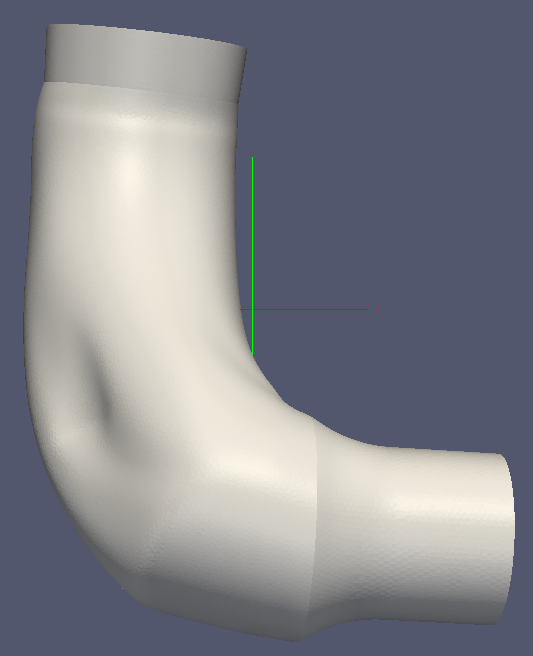
\includegraphics[scale=0.3]{tube_iteration_30}
\end{figure}

\section*{References}
\begin{enumerate}
    \item Mohammadi, Bijan; Pironneau, Olivier. Applied shape optimization for fluids. Second edition. Numerical Mathematics and Scientific Computation. Oxford University Press, Oxford, 2010. xiv+277 pp. ISBN: 978-0-19-954690-9.
    \item Othmer, C. A continuous adjoint formulation for the computation of topological and surface sensitivities of ducted flows. Internat. J. Numer. Methods Fluids 58 (2008), no. 8, 861–877.
    \item Pope, Stephen B. Turbulent flows. Cambridge University Press, Cambridge, 2000. xxxiv+771 pp. ISBN: 0-521-59886-9.
    \item Sokołowski, Jan; Zolésio, Jean-Paul. Introduction to shape optimization. Shape sensitivity analysis. Springer Series in Computational Mathematics, 16. Springer-Verlag, Berlin, 1992. ii+250 pp. ISBN: 3-540-54177-2.
\end{enumerate}

\printbibliography[heading=bibintoc]
\end{document}